%!TEX root = widefieldscan.tex
\svnidlong
{$HeadURL$}
{$LastChangedDate$}
{$LastChangedRevision$}
{$LastChangedBy$}

\ifhtml
\else
\begin{center}
	\fbox{
		\begin{minipage}{.618\columnwidth}
		The section below is versioned at \url{\svnkw{HeadURL}} (last commit @ \svnfileday.\svnfilemonth.\svnfileyear \space \svnfilehour:\svnfileminute, Revision: \svnkw{LastChangedRevision}).
		\end{minipage}
	} 
\end{center}
\fi

\section{Materials and Methods}%
\label{sec:materials and methods}%
\subsection{Sample Preparation and Image Acquisition}%
To validate our theoretical findings and to quantify the achievable resolution, contrast and reduction in acquisition time we used rat lung samples, prepared according  to%
\ifhtml
	~\citet{Schittny1997}
\else
	~\citeasnoun{Schittny1997}
\fi%
\cite{Schittny1998}\todo{citations (taken from Schittny2008) still valid for our protocol?}. Briefly, lungs of Sprague-Dawley rats have been extracted after they have been perfused and filled with phosphate buffered saline by instillation via tracheotomy until the mid respiratory lung volume was reached. Handling of the animals before and during the experiments, as well as the experiments themselves, were approved and supervised by the Swiss Agency for the Environment, Forests and Landscape and the Veterinary Service of the Canton of Bern.

The extracted lung lobes have been fixed in \SI{2.5}{\percent} glutaraldehyde (C$_5$H$_8$O$_2$). For the preparation of the imaging the samples have been postfixed---comparable to electron microscopy protocols---with \SI{1}{\percent} osmium tetroxide (OsO$_4$) and stained with \SI{4}{\percent} uranyl acetate (C$_4$H$_6$O$_6$U), dehydrated in a graded series of ethanol and transferred into paraffin. The lung samples have been mounted onto standard electron microscopy sample mounts with a diameter of approximately \SI{13}{\milli\meter} (PLANO GmbH, Wetzlar, Germany) using paraffin.

\subsection{SRXTM}%
All experiments were performed at the TOMCAT beamline, Swiss Light Source, Paul Scherrer Institut, Villigen, Switzerland. %; , which is located at the X02DA port of the SLS and is one of 17 currently operating beamlines.
TOMCAT receives photons from a \SI{2.9}{\tesla} super-bending magnet. The critical energy of this super-bending magnet is \SI{11.1}{\kilo\electronvolt} (corresponding to a wavelength of \SI{1.22}{\angstrom}). A double crystal multilayer monochromator covers an energy range between 6 and \SI{45}{\kilo\electronvolt} with a bandwidth range of a few percent to a few permille. Detailed technical specifications of the beamline and beam characteristics have been described by%
\ifhtml
	~\citet{Stampanoni2006a}
\else
	~\citeasnoun{Stampanoni2006a}
\fi%
.

\subsubsection{Image acquisition and reconstruction}%
\label{seq:Image Acquisition}%
The samples have been scanned at an x-ray energy of \SI{12.6}{\kilo\electronvolt}. After penetration of the sample, the x-rays are converted into visible light by a YAG:Ce scintillator (\SI{18}{\micro\meter} thickness, Crismatec Saint-Gobain, Nemours, France). The projection images were further magnified by diffraction limited microscope optics and digitized by a high-resolution 2048$\times$2048 pixel CCD camera (pco.2000, PCO AG, Kelheim, Germany) with 14 bit dynamic range. % which can record projections into the internal memory of \SI{4}{\giga\byte}.
The lung samples were imaged using a 10$\times$ magnification, with 2$\times$2 binning and \SI{175}{\milli\second} exposure time resulting in isotropic voxels with a side length of \SI{1.48}{\micro\meter}\todo{no binning for Sophies Sample shown for the 5-subscan-case, hence pixel size \SI{.73}{\micro\meter}}.

Projection images $I_{Pr}$---essentially single radiographies---of the samples have been recorded at several angular positions between \SI{0}{\degree} and \SI{180}{\degree}. The exact number of angular projections depends on the selected scan protocol. Additionally, a set of dark ($I_{D}$) and flat images ($I_{F}$) are recorded for each protocol. The dark images $I_{D}$ were recorded at the start of the scan to capture the noise and dark current of the camera. The flat images $I_{F}$ recorded at the start and at the end of the scan, it capture the beam profile.

Corrected projection images $I_{cPr}$ have been obtained by correcting $I_{Pr}$ with the average dark ($\overline{I_{D}}$) and average flat image ($\overline{I_{F}}$) using the Beer-Lambert law in Equation~\ref{eq:beer-lambert} and relation described in equation~\ref{eq:cpr}.

The Beer--Lambert law relates the absorption of electromagnetic waves to the properties of the material through which these waves are traveling. Let $I_{0}$ and $I_{1}$ be the intensity of the incident electromagnetic wave and the intensity after penetration of the material, respectively. If $\alpha$ describes the absorption coefficient of the substance and $l$ the path length the wave travels through the material, then the intensity of the transmitted wave can be calculated using the Beer--Lambert law: \(I_{1}=I_{0}e^{-\alpha l}\label{eq:beer-lambert}\).

The inversion of the Beer--Lambert law was used to calculate the corrected projection images $I_{cPr}$:
\begin{equation}
	I_{cPr} = -ln\left(\frac{I_{Pr}-\overline{I_{D}}}{\overline{I_{F}}-\overline{I_{D}}}\right)
	= ln(\overline{I_{F}}-\overline{I_{D}})-ln(I_{Pr}-\overline{I_{D}})
	\label{eq:cpr}
\end{equation}

A detailed description of the workflow and the steps necessary to compute a tomographic data set from a set of angular projections can be found in%
\ifhtml
	~\citet{Hintermueller2009}
\else
	~\citeasnoun{Hintermueller2009}
\fi%
.

\subsubsection{Covering a broad FOV}%
\label{subsec:covering a broad fov}%
For parallel beam geometry, tomographic images are obtained at equidistant angles over a sample rotation of \SI{180}{\degree} as shown in figure~\ref{subfig:scanning-possibilities}. After reconstruction the width of the image corresponds to the FOV of the camera.

Samples which are twice as large as the field of view can be imaged using scan protocols based on a \SI{360}{\degree} off-centre sample rotation. After the acquisition half of the images from the dataset have to be flipped and the projections at position $P_{x}$ and $P_{x+\SI{180}{\degree}}$ are stitched together to projection images covering two times the FOV of the camera.

\ifiucr
	%\onecolumn
	\begin{figure}
		\centering
		\caption{a): Covering the FOV of differently sized samples with one \SI{180}{\degree} scan (top), one \SI{360}{\degree} scan (center) or---in the case of the so called wide field scanning---with multiple subscans (three subscans, bottom) The filled red, green and blue segments mark the region of the sample which is covered while scanning the respective positions. b): Increasing the vertical FOV with stacked scanning.}%
		\begin{tabular}{p{.4\linewidth}p{.4\linewidth}}%
			%\documentclass{article}
%\usepackage[demo]{graphicx}
%\usepackage{subfig}
%\usepackage{tikz}
%\usepackage{multirow}
%\usepackage{siunitx}
%\begin{document}
%\begin{figure}
%%%%%%%%%%%%%%%%%%%%%%%%%%%%%
%\begin{tabular}{cc}
%Fig A & \multirow{3}{*}{Fig D}\\
%Fig B & \\
%Fig C & \\
%\end{tabular}
\noindent\makebox[\textwidth]{%
\begin{tabular}{cc}
%%%%% LEFT TOP %%%%%
	\subfloat[\SI{180}{\degree-scan}]{
		%%%%%
		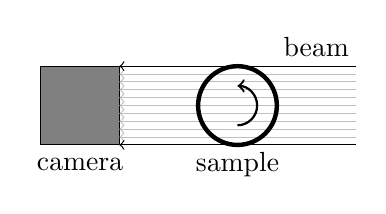
\begin{tikzpicture}
			%drawing grid
			%\draw[color=gray] (0,0) grid (8,1);
			\def\start{0}
			\def\length{1}
			%camera
			\draw [fill=gray] (\start,\start) rectangle (\length,\length);
			\node at (.5*\length,-.25) {camera};
			% beam
			\foreach \x in {0,.1,...,1.1}
				\draw[gray!50,<-] (\length,\x) -- (4*\length,\x);
			\foreach \x in {0,\length}
				\draw[<-] (\length,\x) -- (4*\length,\x);
			\node at (3.5*\length,\length+.25) {beam};
			%sample
			\draw[ultra thick] (2.5*\length,0.5*\length) circle (.5*\length);
			\draw[thick,->] (2.5*\length,0.25*\length) arc (-90:90:.25*\length);
			\node at (2.5*\length,-.25) {sample};
		\end{tikzpicture}
		%%%%%
		\label{subfig:180degreescan}
	}%
& %%%%% RIGHT TOP %%%%%
	\multirow{3}{*}{%
	\subfloat[Stacked scanning for long and thin samples]{
		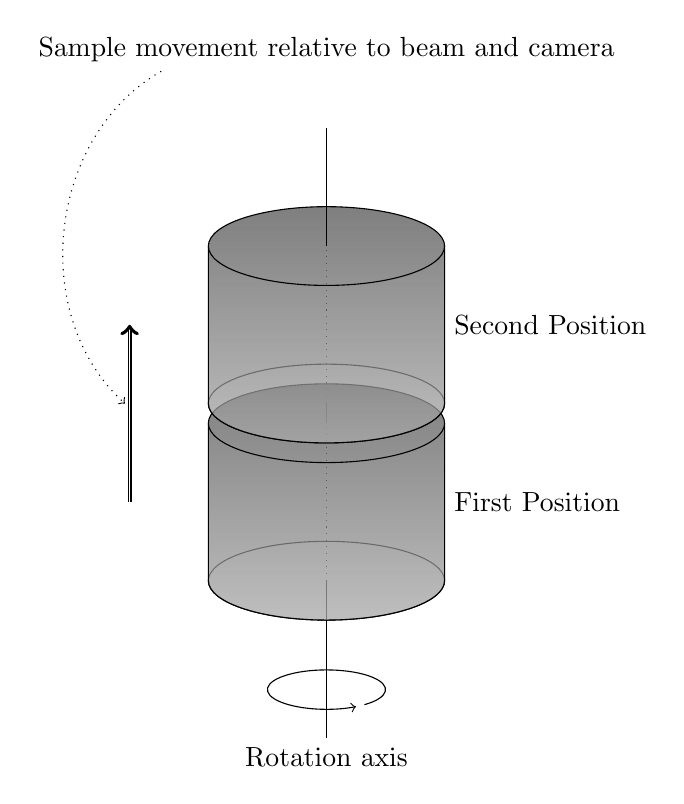
\begin{tikzpicture}%[ultra thick,scale=1]%,show background grid]
			%draw axes
				%\draw[ultra thick] (-10,0) -- (10,0);
				%\draw[ultra thick] (0,-10) -- (0,10);
				%\draw[ultra thick] (0,0) circle (.125);
			% rotation axis
				\draw[->] (0,-2) ++ (-50:.75) arc (-50:300:.75 and .25);
				\draw (0,-3) node [below] {Rotation axis} -- ++(0,2);
				\draw[dotted] (0,-1) -- ++(0,2);
				\draw (0,1) -- ++(0,0.25);
				\draw[dotted] (0,1.25) -- ++(0,2);
			% position 1
				\draw (0,-1) circle (1.5 and .5);
				\fill[shade,semitransparent] (-1.5,-1) arc (-180:0:1.5 and .5) -- ++(0,2) arc (0:180:1.5 and .5) -- cycle;
				\draw (-1.5,-1) arc (-180:0:1.5 and .5) -- ++(0,2) arc (0:180:1.5 and .5) -- cycle;		
				\draw (-1.5,1) arc (-180:0:1.5 and .5);
				\draw (1.5,0) node [right] {First Position};
			% position 2
				\draw (0,1.25) circle (1.5 and .5);
				\fill[shade,semitransparent] (-1.5,1.25) arc (-180:0:1.5 and .5) -- ++(0,2) arc (0:180:1.5 and .5) -- cycle;
				\draw (-1.5,1.25) arc (-180:0:1.5 and .5) -- ++(0,2) arc (0:180:1.5 and .5) -- cycle;		
				\draw (-1.5,3.25) arc (-180:0:1.5 and .5);
				\draw (1.5,2.25) node [right] {Second Position};
			% rotation axis on top
				\draw (0,3.25) -- ++(0,1.5);									
			% sample movement
				\draw[double,->] (-2.5,0) -- (-2.5,2.25) ;% node [text width=10cm,midway,left] {Sample movement relative to beam and camera};	
				% sample movement
				\node (movefrom) at (0,5.75) {Sample movement relative to beam and camera};
				\node (moveto) at (-2.5,1.125) {};
				\draw [->,dotted] (movefrom) to [bend right=54] (moveto);
		\end{tikzpicture}
		\label{subfig:stackedscan}
	}%
	}
\\
%%%%% LEFT MIDDLE %%%%%	
	\subfloat[\SI{360}{\degree-scan}]{
		%%%%%
		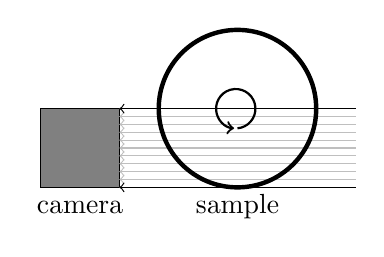
\begin{tikzpicture}
			%drawing grid
			%\draw[color=gray] (0,0) grid (8,1);
			\def\start{0}
			\def\length{1}
			%camera
			\draw [fill=gray] (\start,\start) rectangle (\length,\length);
			\node at (.5*\length,-.25) {camera};
			% beam
			\foreach \x in {0,.1,...,1.1}
				\draw[gray!50,<-] (\length,\x) -- (4*\length,\x);
			\foreach \x in {0,\length}
				\draw[<-] (\length,\x) -- (4*\length,\x);
		%	\node at (3.5*\length,\length+.25) {beam};
			%sample
			\draw[ultra thick] (2.5*\length,\length) circle (\length);
			\draw[thick,->] (2.5*\length,\length-0.25*\length) arc (-85:265:0.25*\length);
			\node at (2.5*\length,-.25) {sample};
		\end{tikzpicture}
		%%%%%
		\label{subfig:360degreescan}
	}%
& %%%%% RIGHT MIDDLE %%%%%
\\
%%%%% LEFT BOTTOMT %%%%%
	\subfloat[wide field scan]{
		%%%%%
		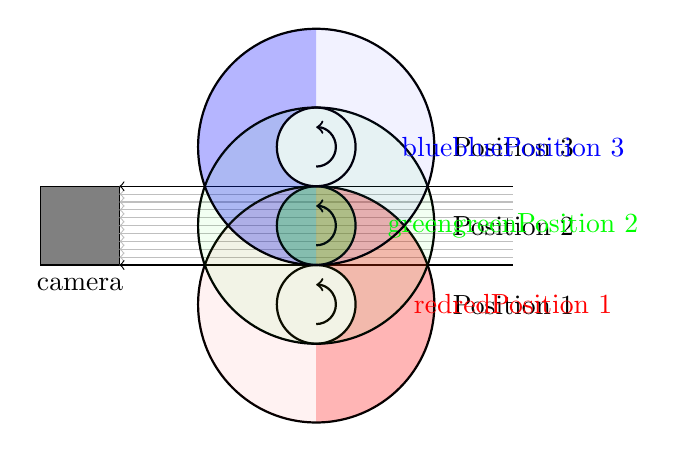
\begin{tikzpicture}
			\def\length{1}
			\def\beamlength{6}
			%grid
		%	\draw[color=gray] (0,-3) grid (7,3);
			%camera
			\draw [fill=gray] (0,0) rectangle (\length,\length);
			\node at (.5*\length,-.25) {camera};
			% beam
			\foreach \x in {0,.1,...,1.1}
				\draw[gray!50,<-] (\length,\x) -- (\beamlength,\x);
			\foreach \x in {0,\length}
				\draw[<-] (\length,\x) -- (\beamlength,\x);
		%	\node at (3.5*\length,\length+.25) {beam};
		%%%%%	%colored samples
		%%%%%	\foreach \y/\color/\position in {-.5/red/1,.5/green/2,1.5/blue/3}
		%%%%%		{
		%%%%%			\draw[thick,color=\color] (0.5*\beamlength+0.5*\length,\y) circle (1.5*\length) circle (.5*\length);
		%%%%%			\draw[thick,->,color=\color] (0.5*\beamlength+0.5*\length,\y-.25*\length) arc (-90:90:0.25*\length);
		%%%%%			\node[color=\color] at (\beamlength,\y) {Position \position};
		%%%%%		}
			% filled samples
			\fill [color=red,nearly transparent]   (3.5,1) arc (90:-90:1.5*\length) -- ++(0,1) arc (-90:90:.5*\length);
			\fill [color=blue,nearly transparent]  (3.5,3) arc (90:270:1.5*\length) -- ++(0,1) arc (270:90:.5*\length);
			\fill [color=green,nearly transparent] (0.5*\beamlength+0.5*\length,.5) circle (0.5*\length);	
			\foreach \y/\position/\color in {-.5/1/red,.5/2/green,1.5/3/blue}
				{
					\draw[thick] (0.5*\beamlength+0.5*\length,\y) circle (1.5*\length) circle (.5*\length);
					\draw[thick,->] (0.5*\beamlength+0.5*\length,\y-.25*\length) arc (-90:90:0.25*\length);
					\fill [color=\color,ultra nearly transparent] (0.5*\beamlength+0.5*\length,\y) circle (1.5*\length);
					\node at (\beamlength+.005,\y-.005) {Position \position};
					\node [color=\color] at (\beamlength,\y) {Position \position};
				}
		\end{tikzpicture}
		%%%%%
		\label{subfig:widefieldscan}
	}%
& %%%%% RIGHT BOTTOM %%%%%
\\
\end{tabular}
} %makebox
%%%%%%%%%%%%%%%%%%%%%%%%%%%%%	
%\caption{Caption of subfigures \subref{subfig:180degreescan}, \subref{subfig:360degreescan}, \subref{subfig:widefieldscan} and \subref{subfig:stackedscan}}
%\end{figure}
%\end{document}%
			\label{subfig:scanning-possibilities}%
		&
			\documentclass{article}
\usepackage[pdftex,active,tightpage]{preview}
\usepackage{tikz}
\usetikzlibrary{arrows,shapes,backgrounds}
\begin{document}
\begin{preview}
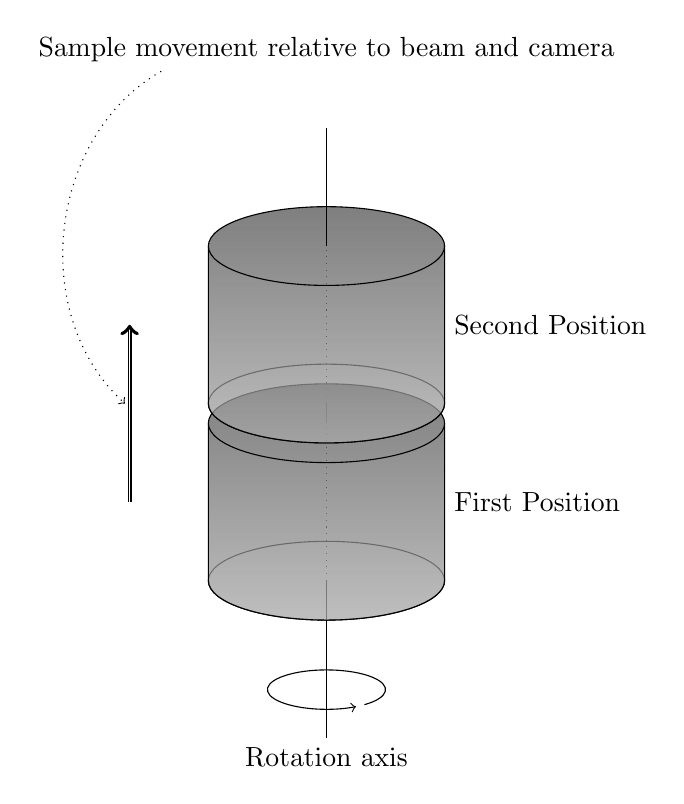
\begin{tikzpicture}%[ultra thick,scale=1]%,show background grid]
	%draw axes
		%\draw[ultra thick] (-10,0) -- (10,0);
		%\draw[ultra thick] (0,-10) -- (0,10);
		%\draw[ultra thick] (0,0) circle (.125);
	% rotation axis
		\draw[->] (0,-2) ++ (-50:.75) arc (-50:300:.75 and .25);
		\draw (0,-3) node [below] {Rotation axis} -- ++(0,2);
		\draw[dotted] (0,-1) -- ++(0,2);
		\draw (0,1) -- ++(0,0.25);
		\draw[dotted] (0,1.25) -- ++(0,2);
	% position 1
		\draw (0,-1) circle (1.5 and .5);
		\fill[shade,semitransparent] (-1.5,-1) arc (-180:0:1.5 and .5) -- ++(0,2) arc (0:180:1.5 and .5) -- cycle;
		\draw (-1.5,-1) arc (-180:0:1.5 and .5) -- ++(0,2) arc (0:180:1.5 and .5) -- cycle;		
		\draw (-1.5,1) arc (-180:0:1.5 and .5);
		\draw (1.5,0) node [right] {First Position};
	% position 2
		\draw (0,1.25) circle (1.5 and .5);
		\fill[shade,semitransparent] (-1.5,1.25) arc (-180:0:1.5 and .5) -- ++(0,2) arc (0:180:1.5 and .5) -- cycle;
		\draw (-1.5,1.25) arc (-180:0:1.5 and .5) -- ++(0,2) arc (0:180:1.5 and .5) -- cycle;		
		\draw (-1.5,3.25) arc (-180:0:1.5 and .5);
		\draw (1.5,2.25) node [right] {Second Position};
	% rotation axis on top
		\draw (0,3.25) -- ++(0,1.5);									
	% sample movement
		\draw[double,->] (-2.5,0) -- (-2.5,2.25) ;% node [text width=10cm,midway,left] {Sample movement relative to beam and camera};	
		% sample movement
		\node (movefrom) at (0,5.75) {Sample movement relative to beam and camera};
		\node (moveto) at (-2.5,1.125) {};
		\draw [->,dotted] (movefrom) to [bend right=54] (moveto);
\end{tikzpicture}
\end{preview}
\end{document}%
			\label{subfig:stacked-scan}%
		\\
			a) Three different scanning configurations for increasing sample diameter.%
		&
			b) Stacked scanning for long and thin samples.%
		\\
		\end{tabular}%
		\label{fig:scanning-possibilities}%
	\end{figure}
	%\twocolumn
\else
	\begin{figure}
		\noindent\makebox[\textwidth]{%
			\subfloat[Three different scanning configurations for increasing sample diameter.]{%
				%\documentclass{article}
%\usepackage[demo]{graphicx}
%\usepackage{subfig}
%\usepackage{tikz}
%\usepackage{multirow}
%\usepackage{siunitx}
%\begin{document}
%\begin{figure}
%%%%%%%%%%%%%%%%%%%%%%%%%%%%%
%\begin{tabular}{cc}
%Fig A & \multirow{3}{*}{Fig D}\\
%Fig B & \\
%Fig C & \\
%\end{tabular}
\noindent\makebox[\textwidth]{%
\begin{tabular}{cc}
%%%%% LEFT TOP %%%%%
	\subfloat[\SI{180}{\degree-scan}]{
		%%%%%
		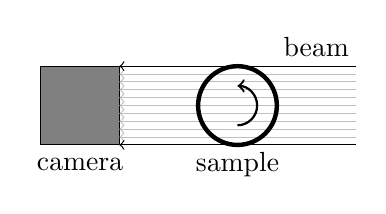
\begin{tikzpicture}
			%drawing grid
			%\draw[color=gray] (0,0) grid (8,1);
			\def\start{0}
			\def\length{1}
			%camera
			\draw [fill=gray] (\start,\start) rectangle (\length,\length);
			\node at (.5*\length,-.25) {camera};
			% beam
			\foreach \x in {0,.1,...,1.1}
				\draw[gray!50,<-] (\length,\x) -- (4*\length,\x);
			\foreach \x in {0,\length}
				\draw[<-] (\length,\x) -- (4*\length,\x);
			\node at (3.5*\length,\length+.25) {beam};
			%sample
			\draw[ultra thick] (2.5*\length,0.5*\length) circle (.5*\length);
			\draw[thick,->] (2.5*\length,0.25*\length) arc (-90:90:.25*\length);
			\node at (2.5*\length,-.25) {sample};
		\end{tikzpicture}
		%%%%%
		\label{subfig:180degreescan}
	}%
& %%%%% RIGHT TOP %%%%%
	\multirow{3}{*}{%
	\subfloat[Stacked scanning for long and thin samples]{
		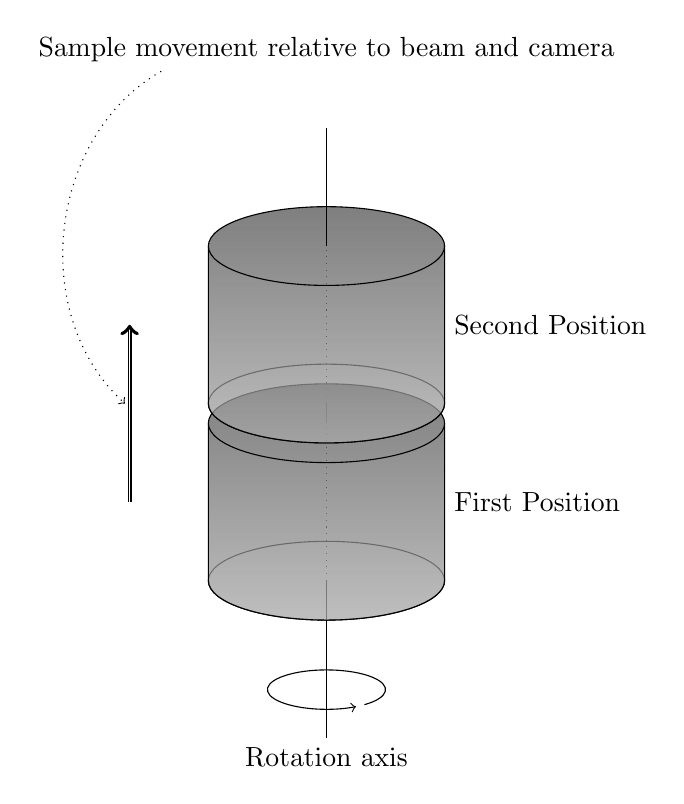
\begin{tikzpicture}%[ultra thick,scale=1]%,show background grid]
			%draw axes
				%\draw[ultra thick] (-10,0) -- (10,0);
				%\draw[ultra thick] (0,-10) -- (0,10);
				%\draw[ultra thick] (0,0) circle (.125);
			% rotation axis
				\draw[->] (0,-2) ++ (-50:.75) arc (-50:300:.75 and .25);
				\draw (0,-3) node [below] {Rotation axis} -- ++(0,2);
				\draw[dotted] (0,-1) -- ++(0,2);
				\draw (0,1) -- ++(0,0.25);
				\draw[dotted] (0,1.25) -- ++(0,2);
			% position 1
				\draw (0,-1) circle (1.5 and .5);
				\fill[shade,semitransparent] (-1.5,-1) arc (-180:0:1.5 and .5) -- ++(0,2) arc (0:180:1.5 and .5) -- cycle;
				\draw (-1.5,-1) arc (-180:0:1.5 and .5) -- ++(0,2) arc (0:180:1.5 and .5) -- cycle;		
				\draw (-1.5,1) arc (-180:0:1.5 and .5);
				\draw (1.5,0) node [right] {First Position};
			% position 2
				\draw (0,1.25) circle (1.5 and .5);
				\fill[shade,semitransparent] (-1.5,1.25) arc (-180:0:1.5 and .5) -- ++(0,2) arc (0:180:1.5 and .5) -- cycle;
				\draw (-1.5,1.25) arc (-180:0:1.5 and .5) -- ++(0,2) arc (0:180:1.5 and .5) -- cycle;		
				\draw (-1.5,3.25) arc (-180:0:1.5 and .5);
				\draw (1.5,2.25) node [right] {Second Position};
			% rotation axis on top
				\draw (0,3.25) -- ++(0,1.5);									
			% sample movement
				\draw[double,->] (-2.5,0) -- (-2.5,2.25) ;% node [text width=10cm,midway,left] {Sample movement relative to beam and camera};	
				% sample movement
				\node (movefrom) at (0,5.75) {Sample movement relative to beam and camera};
				\node (moveto) at (-2.5,1.125) {};
				\draw [->,dotted] (movefrom) to [bend right=54] (moveto);
		\end{tikzpicture}
		\label{subfig:stackedscan}
	}%
	}
\\
%%%%% LEFT MIDDLE %%%%%	
	\subfloat[\SI{360}{\degree-scan}]{
		%%%%%
		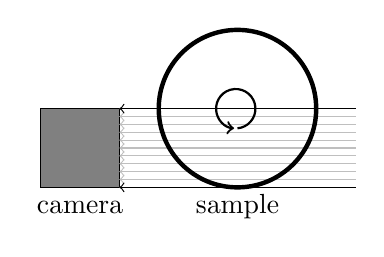
\begin{tikzpicture}
			%drawing grid
			%\draw[color=gray] (0,0) grid (8,1);
			\def\start{0}
			\def\length{1}
			%camera
			\draw [fill=gray] (\start,\start) rectangle (\length,\length);
			\node at (.5*\length,-.25) {camera};
			% beam
			\foreach \x in {0,.1,...,1.1}
				\draw[gray!50,<-] (\length,\x) -- (4*\length,\x);
			\foreach \x in {0,\length}
				\draw[<-] (\length,\x) -- (4*\length,\x);
		%	\node at (3.5*\length,\length+.25) {beam};
			%sample
			\draw[ultra thick] (2.5*\length,\length) circle (\length);
			\draw[thick,->] (2.5*\length,\length-0.25*\length) arc (-85:265:0.25*\length);
			\node at (2.5*\length,-.25) {sample};
		\end{tikzpicture}
		%%%%%
		\label{subfig:360degreescan}
	}%
& %%%%% RIGHT MIDDLE %%%%%
\\
%%%%% LEFT BOTTOMT %%%%%
	\subfloat[wide field scan]{
		%%%%%
		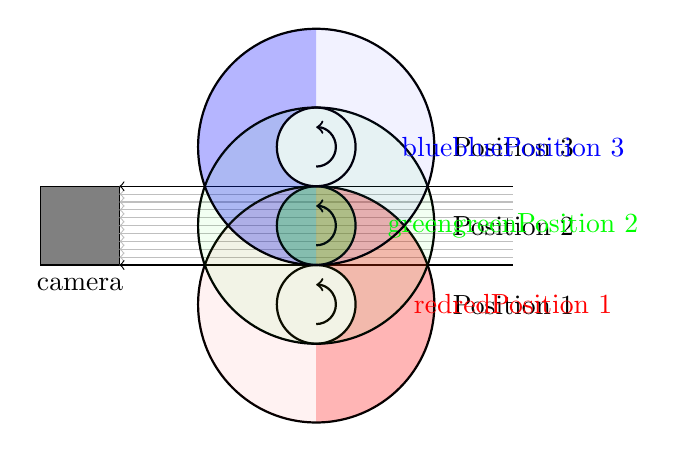
\begin{tikzpicture}
			\def\length{1}
			\def\beamlength{6}
			%grid
		%	\draw[color=gray] (0,-3) grid (7,3);
			%camera
			\draw [fill=gray] (0,0) rectangle (\length,\length);
			\node at (.5*\length,-.25) {camera};
			% beam
			\foreach \x in {0,.1,...,1.1}
				\draw[gray!50,<-] (\length,\x) -- (\beamlength,\x);
			\foreach \x in {0,\length}
				\draw[<-] (\length,\x) -- (\beamlength,\x);
		%	\node at (3.5*\length,\length+.25) {beam};
		%%%%%	%colored samples
		%%%%%	\foreach \y/\color/\position in {-.5/red/1,.5/green/2,1.5/blue/3}
		%%%%%		{
		%%%%%			\draw[thick,color=\color] (0.5*\beamlength+0.5*\length,\y) circle (1.5*\length) circle (.5*\length);
		%%%%%			\draw[thick,->,color=\color] (0.5*\beamlength+0.5*\length,\y-.25*\length) arc (-90:90:0.25*\length);
		%%%%%			\node[color=\color] at (\beamlength,\y) {Position \position};
		%%%%%		}
			% filled samples
			\fill [color=red,nearly transparent]   (3.5,1) arc (90:-90:1.5*\length) -- ++(0,1) arc (-90:90:.5*\length);
			\fill [color=blue,nearly transparent]  (3.5,3) arc (90:270:1.5*\length) -- ++(0,1) arc (270:90:.5*\length);
			\fill [color=green,nearly transparent] (0.5*\beamlength+0.5*\length,.5) circle (0.5*\length);	
			\foreach \y/\position/\color in {-.5/1/red,.5/2/green,1.5/3/blue}
				{
					\draw[thick] (0.5*\beamlength+0.5*\length,\y) circle (1.5*\length) circle (.5*\length);
					\draw[thick,->] (0.5*\beamlength+0.5*\length,\y-.25*\length) arc (-90:90:0.25*\length);
					\fill [color=\color,ultra nearly transparent] (0.5*\beamlength+0.5*\length,\y) circle (1.5*\length);
					\node at (\beamlength+.005,\y-.005) {Position \position};
					\node [color=\color] at (\beamlength,\y) {Position \position};
				}
		\end{tikzpicture}
		%%%%%
		\label{subfig:widefieldscan}
	}%
& %%%%% RIGHT BOTTOM %%%%%
\\
\end{tabular}
} %makebox
%%%%%%%%%%%%%%%%%%%%%%%%%%%%%	
%\caption{Caption of subfigures \subref{subfig:180degreescan}, \subref{subfig:360degreescan}, \subref{subfig:widefieldscan} and \subref{subfig:stackedscan}}
%\end{figure}
%\end{document}%
				\label{subfig:scanning-possibilities}%
			}%
			\subfloat[Stacked scanning for long and thin samples.]{%
				\documentclass{article}
\usepackage[pdftex,active,tightpage]{preview}
\usepackage{tikz}
\usetikzlibrary{arrows,shapes,backgrounds}
\begin{document}
\begin{preview}
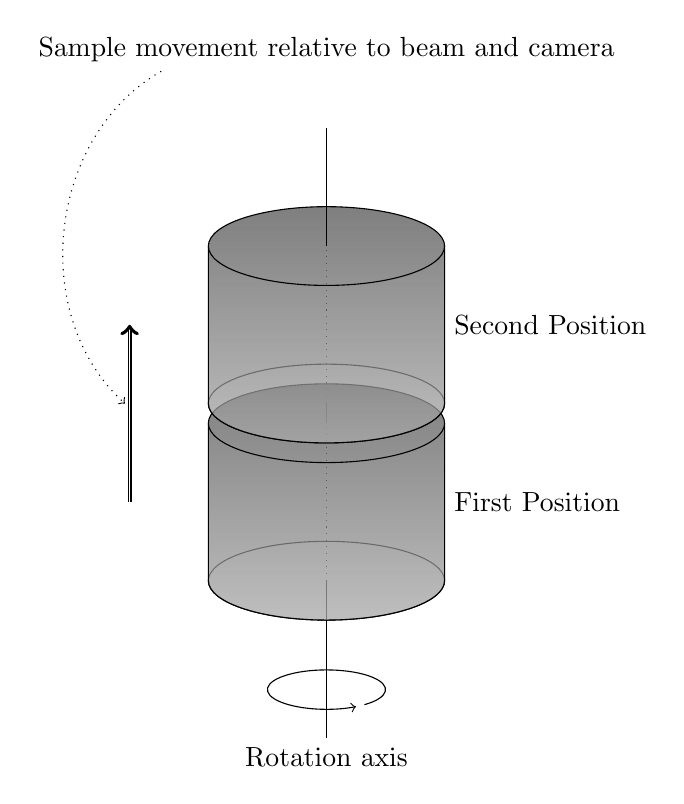
\begin{tikzpicture}%[ultra thick,scale=1]%,show background grid]
	%draw axes
		%\draw[ultra thick] (-10,0) -- (10,0);
		%\draw[ultra thick] (0,-10) -- (0,10);
		%\draw[ultra thick] (0,0) circle (.125);
	% rotation axis
		\draw[->] (0,-2) ++ (-50:.75) arc (-50:300:.75 and .25);
		\draw (0,-3) node [below] {Rotation axis} -- ++(0,2);
		\draw[dotted] (0,-1) -- ++(0,2);
		\draw (0,1) -- ++(0,0.25);
		\draw[dotted] (0,1.25) -- ++(0,2);
	% position 1
		\draw (0,-1) circle (1.5 and .5);
		\fill[shade,semitransparent] (-1.5,-1) arc (-180:0:1.5 and .5) -- ++(0,2) arc (0:180:1.5 and .5) -- cycle;
		\draw (-1.5,-1) arc (-180:0:1.5 and .5) -- ++(0,2) arc (0:180:1.5 and .5) -- cycle;		
		\draw (-1.5,1) arc (-180:0:1.5 and .5);
		\draw (1.5,0) node [right] {First Position};
	% position 2
		\draw (0,1.25) circle (1.5 and .5);
		\fill[shade,semitransparent] (-1.5,1.25) arc (-180:0:1.5 and .5) -- ++(0,2) arc (0:180:1.5 and .5) -- cycle;
		\draw (-1.5,1.25) arc (-180:0:1.5 and .5) -- ++(0,2) arc (0:180:1.5 and .5) -- cycle;		
		\draw (-1.5,3.25) arc (-180:0:1.5 and .5);
		\draw (1.5,2.25) node [right] {Second Position};
	% rotation axis on top
		\draw (0,3.25) -- ++(0,1.5);									
	% sample movement
		\draw[double,->] (-2.5,0) -- (-2.5,2.25) ;% node [text width=10cm,midway,left] {Sample movement relative to beam and camera};	
		% sample movement
		\node (movefrom) at (0,5.75) {Sample movement relative to beam and camera};
		\node (moveto) at (-2.5,1.125) {};
		\draw [->,dotted] (movefrom) to [bend right=54] (moveto);
\end{tikzpicture}
\end{preview}
\end{document}%
				\label{subfig:stacked-scan}%
			}%
		}% end of \makebox
		\caption{\subref{subfig:scanning-possibilities}: Covering the FOV of differently sized samples with one \SI{180}{\degree} scan (top), one \SI{360}{\degree} scan (center) or---in the case of the so called wide field scanning---with multiple subscans (three subscans, bottom) The filled red, green and blue segments mark the region of the sample which is covered while scanning the respective positions. \subref{subfig:stacked-scan}: Increasing the vertical FOV with stacked scanning.
		}%
		\label{fig:scanning-possibilities}%
	\end{figure}
\fi

If we want to achieve tomographic scans covering a sample size which is bigger than what can be achieved with a \SI{360}{\degree}-scan, we have to move the sample in relation to the beam and camera while performing several partial scans. This can be done as shown in figure~\ref{subfig:scanning-possibilities}, where we obtain three subscans to be able to reconstruct a sample as big as three FOVs.

While covering the desired FOV, the projection images of each subscan have to overlap by a few pixels to allow for an optimal stitching of the multiple projections into one big projection. Preliminary experiments have shown that an overlap of approximately 20 pixels allows for the calculation of the cutting line between the independent subscans with a precision of one pixel. Using the mean squared difference between adjacent subscan images~\cite{Hintermueller2009}, such a cutline has been calculated for all the adjacent subscans of every scanned protocol and used to merge the single projections into projections covering the full FOV.

\subsection{Generation of multiple scanning protocols}%
The discussed scanning protocols are generated based on the assumption that a sufficient resolution and contrast can be achieved in the tomographic data sets when the sampling theorem is fulfilled for each sub scan individually. This results in a set of scans with $N_{i}$ images. A simple example with $N_{1}=4$ and $N_{2}=N_{3}=8$ is shown in figure~\ref{fig:projections}.

To be able to reconstruct the sample, we need to stitch the individual sets of projections to projections spanning the desired FOV. Since each scan has a different number of projections $N_{i}$, a stitching algorithm has to interpolate projections from adjacent projections (as shown in figure~\ref{subfig:ProjectionSetupInterpolate}). Alternatively, the same number of projections has to be acquired for all subscans, leading to oversampling for the central scanning position.

\ifiucr
	\begin{figure}%
		\caption{Setup with one central (green) and two lateral scans (red and blue, respectively). For demonstration purposes, the central scan has four projections and the lateral scans have eight projections each (all acquired over \SI{180}{\degree}). The colors of the three positions correspond to the colors shown in figure~\ref{subfig:scanning-possibilities}. a): scanned projections, b): scanned projections and additional interpolated projections (dashed) needed to correctly merge all projections.}%
		\begin{tabular}{cc}%
			%\documentclass{article}
%\usepackage[demo]{graphicx}
%\usepackage{subfig}
%\usepackage{tikz}
%\usepackage{multirow}
%\usepackage{siunitx}
%\begin{document}
%\begin{figure}
%\centering
%%%%%%%%%%%%%%%%%%%%%%%%%%%%%
\def\radius{1}%
\def\gap{0.05}%
\begin{tikzpicture}[ultra thick,scale=.618]%
	\foreach \ang in {0,45,...,359}%
		{%
		\draw [color=green] (\ang:0) -- (\ang:\radius);%
		}%
	\foreach \ang in {0,22.5,...,179}%
		{%
		\draw [color=red] (\ang:\radius+\gap) -- (\ang:3*\radius+\gap);%
		}%
	\foreach \ang in {180,202.5,...,359}%
		{%
		\draw [color=blue] (\ang:\radius+\gap) -- (\ang:3*\radius+\gap);%
		}%
	\node [anchor=south west] at (-3.05,-3.05) {(a)};
\end{tikzpicture}
%%%%%%%%%%%%%%%%%%%%%%%%%%%%%	
%\caption{Projection Setup}
%\end{figure}
%\end{document}%
			\label{subfig:ProjectionSetup}%
		&%
			\input{tikz-images/ProjectionSetupInterpolate}%
			\label{subfig:ProjectionSetupInterpolate}%
		\\%
		a) & b)\\%
		\end{tabular}%
		\label{fig:projections}%
	\end{figure}%
\else
	\begin{figure*}[htp]
		\centering
		\subfloat[]{%
			%\documentclass{article}
%\usepackage[demo]{graphicx}
%\usepackage{subfig}
%\usepackage{tikz}
%\usepackage{multirow}
%\usepackage{siunitx}
%\begin{document}
%\begin{figure}
%\centering
%%%%%%%%%%%%%%%%%%%%%%%%%%%%%
\def\radius{1}%
\def\gap{0.05}%
\begin{tikzpicture}[ultra thick,scale=.618]%
	\foreach \ang in {0,45,...,359}%
		{%
		\draw [color=green] (\ang:0) -- (\ang:\radius);%
		}%
	\foreach \ang in {0,22.5,...,179}%
		{%
		\draw [color=red] (\ang:\radius+\gap) -- (\ang:3*\radius+\gap);%
		}%
	\foreach \ang in {180,202.5,...,359}%
		{%
		\draw [color=blue] (\ang:\radius+\gap) -- (\ang:3*\radius+\gap);%
		}%
	\node [anchor=south west] at (-3.05,-3.05) {(a)};
\end{tikzpicture}
%%%%%%%%%%%%%%%%%%%%%%%%%%%%%	
%\caption{Projection Setup}
%\end{figure}
%\end{document}%
			\label{subfig:ProjectionSetup}%
			}%
		\subfloat[]{%
			\input{tikz-images/ProjectionSetupInterpolate}%
			\label{subfig:ProjectionSetupInterpolate}%
			}%
	%	\caption[Setup with one central and two lateral scans]
		\caption{Setup with one central (green) and two lateral scans (red and blue, respectively). For demonstration purposes, the central scan has four projections and the lateral scans have eight projections each (all acquired over \SI{180}{\degree}). The colors of the three positions correspond to the colors shown in figure~\ref{subfig:scanning-possibilities}. \subref{subfig:ProjectionSetup}: scanned projections, \subref{subfig:ProjectionSetupInterpolate}: scanned projections and additional interpolated projections (dashed) needed to correctly merge all projections.}
		\label{fig:projections}
	\end{figure*}
\fi

\subsubsection{Reduction of the acquisition time}%
Since the total acquisition time per sample linearly scales with the total number of projections and the exposure time, we tend to avoid such an oversampling in the favor of increasing the number of samples which can be imaged during one beamtime. In order to reduce the time required for scanning one single sample compared to a gold standard scan, acquisition protocols with varying amount of projections for each of the three subscans have been designed.

To simplify the interpolation and merging of the projections from each subscan, we selected protocols where the amount of projections from the inner ($N_{inner}$) to the outer subscans ($N_{outer}$) is always a multiple of two: $\frac{N_{outer}}{N_{inner}} \bmod 2 = 0$.

If the amount of projections would not be a multiple of two, stitching the projections of the inner scan with the projections from the outer ones would introduce additional processing steps to interpolate the required intermediate projections. Figure \ref{fig:amount of projections} shows how the projections from the different subscans relate to each other in the more complex case. In this case we would acquire 1500 projections for the central and two times 3000 projections for the two ring-scans to fully satisfy the sampling theorem in each scan while avoiding oversampling of the central scan. 

\ifiucr
	%\onecolumn
	\begin{figure}%
		\caption{Number of merged projections for one central- and two ring-scan. We assume that we have obtained 1500 projections for the central scan and thus acquire two times 1500 projections for each of the lateral scans. This enables us to stitch the projections $P_{1_{284}}$ % XXX XXX 17*3000/180 XXX
	 		(red line) from subscan 1 (ring scan, red area), projection $P_{2_{142}}$ % XXX 17*1500/180 XXX
	 		(green line) from subscan 2 (central scan, green area) and projection $P_{3_{283}}$ % XXX 17*3000/180 XXX
	 		(blue line) of subscan 3 (ring scan, blue area) to one big projection $P_{merge_{284}}$ % XXX 17*3000/180 XXX
			which covers the full FOV. The areas of the three subscans overlap slightly as described above to account for variations in positioning. For illustration purposes we shifted the central projection (green) by \SI{2}{\degree}, otherwise the overlap between these particular projection would not be visible.}%
		%\documentclass{article}
%\usepackage[pdftex,active,tightpage]{preview}
%\usepackage{tikz}
%\begin{document}
%\begin{preview}
	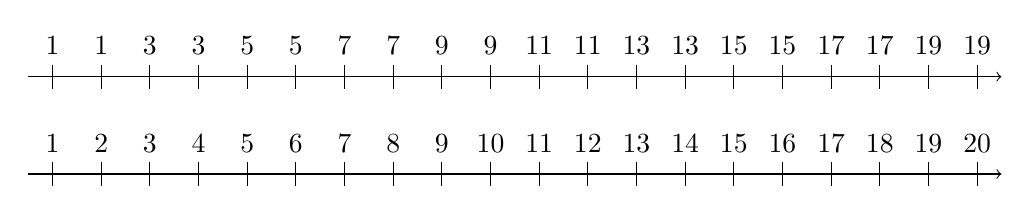
\begin{tikzpicture}[scale=.618]
	\def\length{20}
	\def\height{2}
		\foreach \y in {0,\height}%	
			\draw [->] (0.5,\y) -- (\length+0.5,\y);		
		\foreach \x in {1,...,\length}
			\draw [anchor=south] (\x,-0.25) -- (\x,0.25) node {\x};	
		\foreach \z in {1,3,...,\length}
			\draw [anchor=south] (\z,\height-0.25) -- (\z,\height+0.25) node {\z} (\z+1,\height-0.25) -- (\z+1,\height+0.25) node {\z};	
	\end{tikzpicture}
%\end{preview}
%\end{document}%
		\label{fig:amount of projections}%
	\end{figure}%
	%\twocolumn
\else
	\begin{figure*}[htp]
		\centering
		%\documentclass{article}
%\usepackage[pdftex,active,tightpage]{preview}
%\usepackage{tikz}
%\begin{document}
%\begin{preview}
	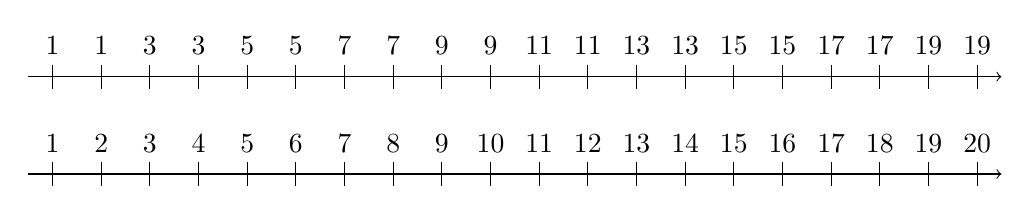
\begin{tikzpicture}[scale=.618]
	\def\length{20}
	\def\height{2}
		\foreach \y in {0,\height}%	
			\draw [->] (0.5,\y) -- (\length+0.5,\y);		
		\foreach \x in {1,...,\length}
			\draw [anchor=south] (\x,-0.25) -- (\x,0.25) node {\x};	
		\foreach \z in {1,3,...,\length}
			\draw [anchor=south] (\z,\height-0.25) -- (\z,\height+0.25) node {\z} (\z+1,\height-0.25) -- (\z+1,\height+0.25) node {\z};	
	\end{tikzpicture}
%\end{preview}
%\end{document}%
	%	\caption[Number of merged projections for one central- and two ring-scan.]
		\caption{Number of merged projections for one central- and two ring-scan. We assume that we have obtained 1500 projections for the central scan and thus acquire two times 1500 projections for each of the lateral scans. This enables us to stitch the projections $P_{1_{284}}$ % XXX XXX 17*3000/180 XXX
	 		(red line) from subscan 1 (ring scan, red area), projection $P_{2_{142}}$ % XXX 17*1500/180 XXX
	 		(green line) from subscan 2 (central scan, green area) and projection $P_{3_{283}}$ % XXX 17*3000/180 XXX
	 		(blue line) of subscan 3 (ring scan, blue area) to one big projection $P_{merge_{284}}$ % XXX 17*3000/180 XXX
			which covers the full FOV. The areas of the three subscans overlap slightly as described above to account for variations in positioning. For illustration purposes we shifted the central projection (green) by \SI{2}{\degree}, otherwise the overlap between these particular projection would not be visible.}%
		\label{fig:amount of projections}%
	\end{figure*}
\fi

\subsubsection{Scanning Time Reduction}%
To be able to further reduce the total scanning time, we developed different scanning protocols, which all relate to a gold standard protocol. Such a gold standard scan would cover the desired FOV while fulfilling the sampling theorem in all parts of the FOV, as shown in figure~\ref{subfig:fovneed3}. For this example we would like to achieve a FOV of 3072$\times$3072 pixels. The dark gray circle shown in aforementioned figure is the FOV that can be fully covered, the rest of the slice in light grey would be either missing or show artifacts arising from partial volume effects, depending on the chosen reconstruction algorithm. To cover this desired FOV with a standard scan obtained from a detector with the size of 1024 pixels, nine independent scans would be needed. Acquiring nine independent scans would show exactly the same ratio of coverage vs.\ potentially missing parts, but some of the missing parts would be lying inside the desired FOV (light gray parts of figure~\ref{subfig:goldstandard3} inside the ring covering the desired FOV). Nonetheless, this setup corresponds to the gold standard scan which has been defined as protocol A in table~\ref{tab:protocols}. Figure~\ref{subfig:protocol3} shows how the desired FOV can be covered with a wide-field scan obtained from merged projections as described above. No missing parts arising from partial volume effects are lying inside the desired FOV.

To fully satisfy the sampling theorem for a scan with the detector width $D$ we need to acquire an amount of projections $P=D\frac{\pi}{2}$, which leads to the acquisition of totally 14476 projections for the setup shown in figure~\ref{subfig:goldstandard3}. For the scan shown in figure~\ref{subfig:protocol3} we also need to acquire 14476 projections, since we need to acquire three times $3072\frac{\pi}{2}$ projections if the single projections from each subscan are to be merged into one projections covering the FOV prior to reconstruction.

\ifiucr
	%\onecolumn
	\begin{figure}%
		\centering%
		\caption{Setup; desired FOV and two variants of covering the desired FOV with 9 independent small scans or 3 subscans.}%
		\begin{tabular}{p{0.3\linewidth}p{0.3\linewidth}p{0.3\linewidth}}
				%\documentclass{article}
%\usepackage{subfig}
%\usepackage{tikz}
%\begin{document}
%\begin{figure}
%\centering
%%%%%%%%%%%%%%%%%%%%%%%%%%%%%
\def\scale{0.45} % -> (3*.44=1.32)
\def\size{3}
%FOV to be covered
	\label{subfig:fovneed3}%
	\begin{tikzpicture}[scale=\scale]
	%	\draw [dashed] (-1,-1) grid (7,7);
		\draw [fill=gray!25] (0,0) rectangle (2*\size,2*\size);
		\fill [semitransparent] (\size,\size) circle (\size);
		\draw (\size,\size) circle (\size);
		\draw [white,ultra thick,<->] (0,\size) -- node [above] {3072 px} (2*\size,\size);
	%	\draw [step=2] (0,0) grid (6,6);
	\end{tikzpicture}%
%%%%%%%%%%%%%%%%%%%%%%%%%%%%%
%\caption{Projection Setup}
%\end{figure}
%\end{document} &%
			\input{tikz-images/SubScanSetup/3gold} &%
			%\documentclass{article}
%\usepackage{subfig}
%\usepackage{tikz}
%\begin{document}
%\begin{figure}
%\centering
%%%%%%%%%%%%%%%%%%%%%%%%%%%%% 3 SUBSCANS %%%%%%%%%%%%%%%%%%%%%%%%%%%%%
\def\scale{0.65} % -> (3*.65=1.95)
\def\size{3}
%Covering the FOV with merged projections from one central and two ring scans.
	\label{subfig:protocol3}%
	\begin{tikzpicture}[scale=\scale]
%		\draw [dashed] (-1,-1) grid (7,7);
		\draw [fill=gray!25] (0,0) rectangle (2*\size,2*\size);
		\fill [semitransparent] (\size,\size) circle (\size);
		\foreach \r in {1,3}
			\draw (\size,\size) circle (\r);
		\draw (0,\size) -- (\size-1,\size);
		\draw (\size+1,\size) -- (2*\size,\size);
		\node at (\size,1) {r1};
		\node at (\size,3) {central};
		\node at (\size,5) {r2};
		\def\angle{155}
		\draw [white,ultra thick,<->] (\size,\size) +(\angle:1) -- node [sloped,midway,above] {1024 px} +(\angle:3); 
	\end{tikzpicture}
%%%%%%%%%%%%%%%%%%%%%%%%%%%%%	
%\caption{Projection Setup}
%\end{figure}
%\end{document}\\%
			a) FOV to be covered &%
			b) Gold Standard; covering the FOV with 9 independently reconstructed small scans&%
			c) Covering the FOV with merged projections from one central and two ring scans\\%
		\end{tabular}%
		\label{fig:Setup3SubScans}%
	\end{figure}%
	%\twocolumn
\else
	\begin{figure*}[htp]
		\centering%
		\input{tikz-images/Setup3SubScans}%
		\caption{Setup; desired FOV and two variants of covering the desired FOV with 9 independent small scans or 3 subscans.}%
		\label{fig:Setup3SubScans}%
	\end{figure*}
\fi

The protocols shown for increasing the FOV to three times the detector width can be iterated to bigger FOV. Figures~\ref{fig:Setup5SubScans} and \ref{fig:Setup7SubScans} show the setup if the FOV has to be increased five or seven times, respectively.

\ifiucr
	\begin{figure}%
		\centering%
		\caption{Setup; desired FOV and two variants of covering the desired FOV with 25 independent small scans or 5 subscans.}%
		\begin{tabular}{p{0.3\linewidth}p{0.3\linewidth}p{0.3\linewidth}}%
			%\documentclass{article}
%\usepackage{subfig}
%\usepackage{tikz}
%\begin{document}
%\begin{figure}
%\centering
%%%%%%%%%%%%%%%%%%%%%%%%%%%%% 5 SUBSCANS %%%%%%%%%%%%%%%%%%%%%%%%%%%%%
\def\scale{0.39} % 1.95/5
\def\size{5}
%FOV to be covered
	\label{subfig:fovneed5}%
	\begin{tikzpicture}[scale=\scale]
	%	\draw [dashed] (-1,-1) grid (7,7);
		\draw [fill=gray!25] (0,0) rectangle (2*\size,2*\size);
		\fill [semitransparent] (\size,\size) circle (\size);
		\draw (\size,\size) circle (\size);
		\draw [white,ultra thick,<->] (0,\size) -- node [above] {5120 px} (2*\size,\size);
	%	\draw [step=2] (0,0) grid (6,6);
	\end{tikzpicture}%
%%%%%%%%%%%%%%%%%%%%%%%%%%%%%	
%\caption{Projection Setup}
%\end{figure}
%\end{document} &%
			\input{tikz-images/SubScanSetup/5gold} &%
			%\documentclass{article}
%\usepackage{subfig}
%\usepackage{tikz}
%\begin{document}
%\begin{figure}
%\centering
\def\scale{0.264} % 1.32/5
\def\size{5}
%Covering the FOV with merged projections from one central and four ring scans.
	\label{subfig:protocol5}%
	\begin{tikzpicture}[scale=\scale]
%		\draw [dashed] (-1,-1) grid (7,7);
		\draw [fill=gray!25] (0,0) rectangle (2*\size,2*\size);
		\fill [semitransparent] (\size,\size) circle (\size);
		\foreach \r in {1,3,5}
			\draw (\size,\size) circle (\r);
		\draw (0,\size) -- (\size-1,\size);
		\draw (\size+1,\size) -- (2*\size,\size);
		\node at (\size,1) {r3};
		\node at (\size,3) {r1};
		\node at (\size,5) {central};
		\node at (\size,7) {r2};
		\node at (\size,9) {r4};
		\def\angle{155}
		\draw [white,ultra thick,<->] (\size,\size) +(\angle:1) -- node [sloped,midway,above] {1024 px} +(\angle:3); 
	\end{tikzpicture}
%%%%%%%%%%%%%%%%%%%%%%%%%%%%%	
%\caption{Projection Setup}
%\end{figure}
%\end{document}\\%
			a) FOV to be covered &%
			b) Gold Standard; covering the FOV with 25 independently reconstructed small scans &%
			c) Covering the FOV with merged projections from one central and four ring scans \\%
		\end{tabular}%
		\label{fig:Setup5SubScans}%
	\end{figure}%
\else
	\begin{figure*}[htp]
		\centering%
		\input{tikz-images/Setup5SubScans}%
	%	\caption[Setup for 5 SubScans]
		\caption{Setup; desired FOV and two variants of covering the desired FOV with 25 independent small scans or 5 subscans.}%
		\label{fig:Setup5SubScans}%
	\end{figure*}
\fi

\ifiucr
	%\onecolumn
	\begin{figure}%
		\centering%
		\caption{Setup; desired FOV and two variants of covering the desired FOV with 49 independent small scans or 7 subscans.}%
		\begin{tabular}{p{0.3\linewidth}p{0.3\linewidth}p{0.3\linewidth}}%
			%\documentclass{article}
%\usepackage{subfig}
%\usepackage{tikz}
%\begin{document}
%\begin{figure}
%\centering
%%%%%%%%%%%%%%%%%%%%%%%%%%%%% 7 SUBSCANS %%%%%%%%%%%%%%%%%%%%%%%%%%%%%
\def\scale{0.18857142857142857142857142857143} % 1.32/7
\def\size{7}
%FOV to be covered%
	\label{subfig:fovneed7}%
	\begin{tikzpicture}[scale=\scale]
	%	\draw [dashed] (-1,-1) grid (7,7);
		\draw [fill=gray!25] (0,0) rectangle (2*\size,2*\size);
		\fill [semitransparent] (\size,\size) circle (\size);
		\draw (\size,\size) circle (\size);
		\draw [white,ultra thick,<->] (0,\size) -- node [above] {7168 px} (2*\size,\size);
	%	\draw [step=2] (0,0) grid (6,6);
	\end{tikzpicture}%
%%%%%%%%%%%%%%%%%%%%%%%%%%%%%	
%\caption{Projection Setup}
%\end{figure}
%\end{document} &%
			%\documentclass{article}
%\usepackage{subfig}
%\usepackage{tikz}
%\begin{document}
%\begin{figure}
%\centering
%%%%%%%%%%%%%%%%%%%%%%%%%%%%% 7 SUBSCANS %%%%%%%%%%%%%%%%%%%%%%%%%%%%%
\def\scale{0.27857142857142857142857142857143} % 1.95/7
\def\size{7}
%Gold Standard; covering the FOV with 49 independently reconstructed small scans.
	\label{subfig:goldstandard7}%
	\begin{tikzpicture}[scale=\scale]
	%	\draw [dashed] (-1,-1) grid (7,7);
		\fill [color=gray!25] (0,0) rectangle (2*\size,2*\size);
		\foreach \x in {1,2,3,4,5,6,7}
			\foreach \y in {1,2,3,4,5,6,7}
				\draw [fill=gray] (2*\x-1,2*\y-1) circle (1) node {\x,\y};
		\fill [semitransparent] (\size,\size) circle (\size);
		\draw (\size,\size) circle (\size);
		\draw [step=2] (0,0) grid (2*\size,2*\size);
		\draw [white,ultra thick,<->] (\size-1,1.1*\size) -- node [above] {1024 px} (\size+1,1.1*\size);
	\end{tikzpicture}%
%%%%%%%%%%%%%%%%%%%%%%%%%%%%%	
%\caption{Projection Setup}
%\end{figure}
%\end{document} &%
			%\documentclass{article}
%\usepackage{subfig}
%\usepackage{tikz}
%\begin{document}
%\begin{figure}
%\centering
%%%%%%%%%%%%%%%%%%%%%%%%%%%%% 7 SUBSCANS %%%%%%%%%%%%%%%%%%%%%%%%%%%%%
\def\scale{0.27857142857142857142857142857143} % 1.95/7
\def\size{7}
%Covering the FOV with merged projections from one central and six ring scans.
	\label{subfig:protocol7}%
	\begin{tikzpicture}[scale=\scale]
%		\draw [dashed] (-1,-1) grid (7,7);
		\draw [fill=gray!25] (0,0) rectangle (2*\size,2*\size);
		\fill [semitransparent] (\size,\size) circle (\size);
		\foreach \r in {1,3,5,7}
			\draw (\size,\size) circle (\r);
		\draw (0,\size) -- (\size-1,\size);
		\draw (\size+1,\size) -- (2*\size,\size);
		\node at (\size,1) {r5};
		\node at (\size,3) {r3};
		\node at (\size,5) {r1};
		\node at (\size,7) {central};
		\node at (\size,9) {r2};
		\node at (\size,11) {r4};
		\node at (\size,13) {r6};
		\def\angle{155}
		\draw [white,ultra thick,<->] (\size,\size) +(\angle:1) -- node [sloped,midway,above] {1024 px} +(\angle:3); 
	\end{tikzpicture}
%%%%%%%%%%%%%%%%%%%%%%%%%%%%%	
%\caption{Projection Setup}
%\end{figure}
%\end{document} \\%
			a) FOV to be covered &%
			b) Gold Standard; covering the FOV with 49 independently reconstructed small scans &%
			c) Covering the FOV with merged projections from one central and six ring scans \\%
		\end{tabular}%
		\label{fig:Setup7SubScans}%
	\end{figure}%
	%\twocolumn
\else
	\begin{figure*}[htp]
		\centering%
		%\documentclass{article}
%\usepackage{subfig}
%\usepackage{tikz}
%\begin{document}
%\begin{figure}
%\centering
%%%%%%%%%%%%%%%%%%%%%%%%%%%%% 3 SUBSCANS %%%%%%%%%%%%%%%%%%%%%%%%%%%%%
%\def\scale{0.65} % -> (3*.65=1.95)
%\def\size{3}
%\subfloat[FOV to be covered]{%
%	\label{subfig:fovneed3}%
%	\begin{tikzpicture}[scale=\scale]
%	%	\draw [dashed] (-1,-1) grid (7,7);
%		\draw [fill=gray!25] (0,0) rectangle (2*\size,2*\size);
%		\fill [semitransparent] (\size,\size) circle (\size);
%		\draw (\size,\size) circle (\size);
%		\draw [white,ultra thick,<->] (0,\size) -- node [above] {3072 px} (2*\size,\size);
%	%	\draw [step=2] (0,0) grid (6,6);
%	\end{tikzpicture}%
%}\hfill
%\subfloat[Gold Standard; covering the FOV with 9 independently reconstructed small scans.]{%
%	\label{subfig:goldstandard3}%
%	\begin{tikzpicture}[scale=\scale]
%	%	\draw [dashed] (-1,-1) grid (7,7);
%		\fill [color=gray!25] (0,0) rectangle (2*\size,2*\size);
%		\foreach \x in {1,2,3}
%			\foreach \y in {1,2,3}
%				\draw [fill=gray] (2*\x-1,2*\y-1) circle (1) node {\x,\y};
%		\fill [semitransparent] (\size,\size) circle (\size);
%		\draw (\size,\size) circle (\size);
%		\draw [step=2] (0,0) grid (2*\size,2*\size);
%		\draw [white,ultra thick,<->] (\size-1,1.1*\size) -- node [above] {1024 px} (\size+1,1.1*\size);
%	\end{tikzpicture}%
%}\hfill
%\subfloat[Covering the FOV with merged projections from one central and two ring scans.]{%
%	\label{subfig:protocol3}%
%	\begin{tikzpicture}[scale=\scale]
%%		\draw [dashed] (-1,-1) grid (7,7);
%		\draw [fill=gray!25] (0,0) rectangle (2*\size,2*\size);
%		\fill [semitransparent] (\size,\size) circle (\size);
%		\foreach \r in {1,3}
%			\draw (\size,\size) circle (\r);
%		\draw (0,\size) -- (\size-1,\size);
%		\draw (\size+1,\size) -- (2*\size,\size);
%		\node at (\size,1) {r1};
%		\node at (\size,3) {central};
%		\node at (\size,5) {r2};
%		\def\angle{155}
%		\draw [white,ultra thick,<->] (\size,\size) +(\angle:1) -- node [sloped,midway,above] {1024 px} +(\angle:3); 
%	\end{tikzpicture}
%}
%%%%%%%%%%%%%%%%%%%%%%%%%%%%%% 3 SUBSCANS %%%%%%%%%%%%%%%%%%%%%%%%%%%%%
%%%%%%%%%%%%%%%%%%%%%%%%%%%%%% 5 SUBSCANS %%%%%%%%%%%%%%%%%%%%%%%%%%%%%
%\def\scale{0.39} % 1.95/5
%\def\size{5}
%\subfloat[FOV to be covered]{%
%	\label{subfig:fovneed5}%
%	\begin{tikzpicture}[scale=\scale]
%	%	\draw [dashed] (-1,-1) grid (7,7);
%		\draw [fill=gray!25] (0,0) rectangle (2*\size,2*\size);
%		\fill [semitransparent] (\size,\size) circle (\size);
%		\draw (\size,\size) circle (\size);
%		\draw [white,ultra thick,<->] (0,\size) -- node [above] {5120 px} (2*\size,\size);
%	%	\draw [step=2] (0,0) grid (6,6);
%	\end{tikzpicture}%
%}\hfill
%\subfloat[Gold Standard; covering the FOV with 25 independently reconstructed small scans.]{%
%	\label{subfig:goldstandard5}%
%	\begin{tikzpicture}[scale=\scale]
%	%	\draw [dashed] (-1,-1) grid (7,7);
%		\fill [color=gray!25] (0,0) rectangle (2*\size,2*\size);
%		\foreach \x in {1,2,3,4,5}
%			\foreach \y in {1,2,3,4,5}
%				\draw [fill=gray] (2*\x-1,2*\y-1) circle (1) node {\x,\y};
%		\fill [semitransparent] (\size,\size) circle (\size);
%		\draw (\size,\size) circle (\size);
%		\draw [step=2] (0,0) grid (2*\size,2*\size);
%		\draw [white,ultra thick,<->] (\size-1,1.1*\size) -- node [above] {1024 px} (\size+1,1.1*\size);
%	\end{tikzpicture}%
%}\hfill
%\subfloat[Covering the FOV with merged projections from one central and four ring scans.]{%
%	\label{subfig:protocol5}%
%	\begin{tikzpicture}[scale=\scale]
%%		\draw [dashed] (-1,-1) grid (7,7);
%		\draw [fill=gray!25] (0,0) rectangle (2*\size,2*\size);
%		\fill [semitransparent] (\size,\size) circle (\size);
%		\foreach \r in {1,3,5}
%			\draw (\size,\size) circle (\r);
%		\draw (0,\size) -- (\size-1,\size);
%		\draw (\size+1,\size) -- (2*\size,\size);
%		\node at (\size,1) {r3};
%		\node at (\size,3) {r1};
%		\node at (\size,5) {central};
%		\node at (\size,7) {r2};
%		\node at (\size,9) {r4};
%		\def\angle{155}
%		\draw [white,ultra thick,<->] (\size,\size) +(\angle:1) -- node [sloped,midway,above] {1024 px} +(\angle:3); 
%	\end{tikzpicture}
%}
%%%%%%%%%%%%%%%%%%%%%%%%%%%%%% 5 SUBSCANS %%%%%%%%%%%%%%%%%%%%%%%%%%%%%
%%%%%%%%%%%%%%%%%%%%%%%%%%%%% 7 SUBSCANS %%%%%%%%%%%%%%%%%%%%%%%%%%%%%
\def\scale{0.27857142857142857142857142857143} % 1.95/7
\def\size{7}
\subfloat[FOV to be covered]{%
	\label{subfig:fovneed7}%
	\begin{tikzpicture}[scale=\scale]
	%	\draw [dashed] (-1,-1) grid (7,7);
		\draw [fill=gray!25] (0,0) rectangle (2*\size,2*\size);
		\fill [semitransparent] (\size,\size) circle (\size);
		\draw (\size,\size) circle (\size);
		\draw [white,ultra thick,<->] (0,\size) -- node [above] {7168 px} (2*\size,\size);
	%	\draw [step=2] (0,0) grid (6,6);
	\end{tikzpicture}%
}\hfill
\subfloat[Gold Standard; covering the FOV with 49 independently reconstructed small scans.]{%
	\label{subfig:goldstandard7}%
	\begin{tikzpicture}[scale=\scale]
	%	\draw [dashed] (-1,-1) grid (7,7);
		\fill [color=gray!25] (0,0) rectangle (2*\size,2*\size);
		\foreach \x in {1,2,3,4,5,6,7}
			\foreach \y in {1,2,3,4,5,6,7}
				\draw [fill=gray] (2*\x-1,2*\y-1) circle (1) node {\x,\y};
		\fill [semitransparent] (\size,\size) circle (\size);
		\draw (\size,\size) circle (\size);
		\draw [step=2] (0,0) grid (2*\size,2*\size);
		\draw [white,ultra thick,<->] (\size-1,1.1*\size) -- node [above] {1024 px} (\size+1,1.1*\size);
	\end{tikzpicture}%
}\hfill
\subfloat[Covering the FOV with merged projections from one central and six ring scans.]{%
	\label{subfig:protocol7}%
	\begin{tikzpicture}[scale=\scale]
%		\draw [dashed] (-1,-1) grid (7,7);
		\draw [fill=gray!25] (0,0) rectangle (2*\size,2*\size);
		\fill [semitransparent] (\size,\size) circle (\size);
		\foreach \r in {1,3,5,7}
			\draw (\size,\size) circle (\r);
		\draw (0,\size) -- (\size-1,\size);
		\draw (\size+1,\size) -- (2*\size,\size);
		\node at (\size,1) {r5};
		\node at (\size,3) {r3};
		\node at (\size,5) {r1};
		\node at (\size,7) {central};
		\node at (\size,9) {r2};
		\node at (\size,11) {r4};
		\node at (\size,13) {r6};
		\def\angle{155}
		\draw [white,ultra thick,<->] (\size,\size) +(\angle:1) -- node [sloped,midway,above] {1024 px} +(\angle:3); 
	\end{tikzpicture}
}
%%%%%%%%%%%%%%%%%%%%%%%%%%%%% 7 SUBSCANS %%%%%%%%%%%%%%%%%%%%%%%%%%%%%
%%%%%%%%%%%%%%%%%%%%%%%%%%%%%	
%\caption{Projection Setup}
%\end{figure}
%\end{document}%
	%	\caption[Setup for 7 SubScans]
		\caption{Setup; desired FOV and two variants of covering the desired FOV with 49 independent small scans or 7 subscans.}%
		\label{fig:Setup7SubScans}%
	\end{figure*}
\fi

\subsection{Wide Field Scanning Setup}%
\label{subsec:wfs-setup}%
A custom MATLAB-script (MATLAB\textsuperscript{\textregistered} 7.6.0.321 (R2008a), The MathWorks, Inc.) has been written to enable the user to input the scanning parameters like desired FOV, detector width, desired overlap between the subscans, magnification and binning. According to these presets, the scripts calculated the necessary projections to fulfill the sampling theorem for the chosen FOV as a gold-standard and computes different acquisition protocols with reduced amount of projections. For all these scanning protocols a reconstruction is simulated using a Shepp-Logan phantom~\cite{Shepp1974} and we calculate the expected reconstruction quality using the difference image for each simulated reconstruction with the gold standard (the original phantom). This expected reconstruction quality is then plotted against the acquisition time, such a plot is shown in figure~\ref{fig:qualityplot}.

After the user has chosen a suitable protocol which balances the requirements for reconstruction quality and need for fast acquisition time (corresponding to one dot in figure~\ref{fig:qualityplot}), a preference file is written. This preference file contains the details of the selected scan like amount of needed subscans, the positions of the sample, number of projections as well as start and stop angles of the rotation for each subscan. Subsequently, the preference file is parsed by a custom Python-script to interact with the EPICS-System (Experimental Physics and Industrial Control System, Argonne National Laboratory, Argonne, USA, \url{http://www.aps.anl.gov/epics/}), which itself is used to control the hardware of the TOMCAT beamline, allowing for an unattended batch scan of all the desired subscans.

After the multiple subscans have been recorded, the stitching of the different amount of projections recorded per subscans into big projections covering the desired FOV is performed with minimal user interaction using a second MATLAB-script. Further processing of the merged projections like sinogram generation and reconstruction into the tomographic dataset is integrated into the TOMCAT data-processing pipeline, as specified by%
\ifhtml
	~\citet{Hintermueller2009}
\else
	~\citeasnoun{Hintermueller2009}
\fi%
).

\ifiucr
	\begin{figure}%
		\centering%
		\caption{Quality-Plot of 19 calculated protocols. The red dots show the expected quality of the different protocols, the black plot is a polynomial fit $p(x)$ with $n=4$ for $p(x)=p_{1}x^{n}+p_{2}x^{n-1}+\cdots+p_{n}x+p_{n+1}$. Details of these scans are shown in table~\ref{tab:protocols} and are discussed in section~\ref{sec:Results}.}%
		%%\documentclass{article}
%\usepackage{tikz,pgfplots}
%\usepackage[pdftex,active,tightpage]{preview}
%\begin{document}
%\begin{preview}
%%%%%%%%%%%%%%%%%%%%%%%%%%%%%%%%%%
%%%%%%%%%%%%%%%%%%%%%%%%%%%%%%%%%%%%%%%%%%%%%%%%%%%%%%%%%%%%%%%%%%%%%%%%%%%%%%%%%%%%%%%%%%%%%%%%%%%%
%%% Obtained with ..MATLAB/WideFieldScan/Paper/QualityPlotPaper.m for a SimluationSize of 1000px %%%
%%%%%%%%%%%%%%%%%%%%%%%%%%%%%%%%%%%%%%%%%%%%%%%%%%%%%%%%%%%%%%%%%%%%%%%%%%%%%%%%%%%%%%%%%%%%%%%%%%%%
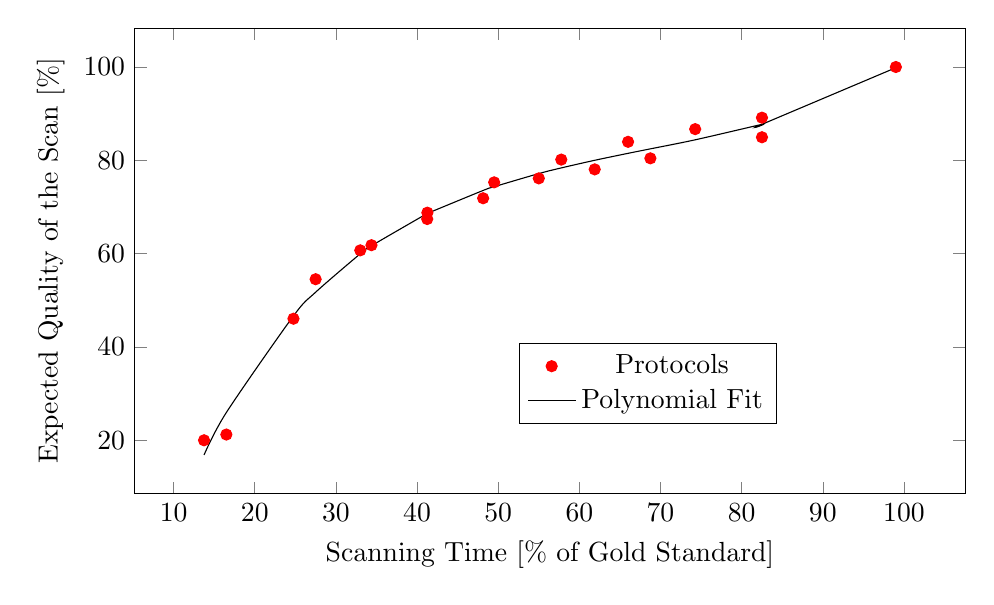
\begin{tikzpicture}

% defining custom colors
\definecolor{mycolor1}{rgb}{0,0.5,0}

\begin{axis}[%
	width=\linewidth,
	height=0.618\linewidth,
%	title={QualityPlot},%
	xlabel={Scanning Time [\%\ of Gold Standard]},%
	ylabel={Expected Quality of the Scan [\%]},%
	]

% Protocols
\addplot [ color = red, only marks, mark = *] 
coordinates{
 (13.7508,20) (16.5009,21.2284) (24.7703,46.0522) (27.5016,54.5201) (33.0019,60.7072) (34.3801,61.8107) (41.2524,67.4167) (41.2712,68.7811) (48.1435,71.8724) (49.5028,75.28) (55.0031,76.1345) (57.7722,80.1592) (61.8943,78.0612) (66.0038,83.9645) (68.7539,80.4284) (74.2731,86.6889) (82.5047,84.9458) (82.5047,89.1421) (99.0057,100)
};

% Line plot
\addplot [smooth, solid]
coordinates{
 (13.7508,16.8548) (16.5009,25.9575) (24.7703,46.6567) (27.5016,51.7347) (33.0019,59.9714) (34.3801,61.6854) (41.2524,68.6146) (41.2712,68.6305) (48.1435,73.5452) (49.5028,74.3455) (55.0031,77.1605) (57.7722,78.3754) (61.8943,80.0091) (66.0038,81.5005) (68.7539,82.4599) (74.2731,84.3973) (82.5047,87.719) (82.5047,87.719) (99.0057,99.8565)
};

\pgfplotsset{every axis legend/.append style={
at={(0.618,0.2)},
anchor=base}}

\legend{Protocols,Polynomial Fit}%$p(x)=p_{1}x^{n}+p_{2}x^{n-1}+...+p_{n}x+p_{n+1}$}

\end{axis}

\end{tikzpicture}
%%%%%%%%%%%%%%%%%%%%%%%%%%%%%%%%%%
%\end{preview}
%\end{document}%
		\label{fig:qualityplot}%
	\end{figure}%
\else
\begin{figure*}[htp]
	\centering%
	%%\documentclass{article}
%\usepackage{tikz,pgfplots}
%\usepackage[pdftex,active,tightpage]{preview}
%\begin{document}
%\begin{preview}
%%%%%%%%%%%%%%%%%%%%%%%%%%%%%%%%%%
%%%%%%%%%%%%%%%%%%%%%%%%%%%%%%%%%%%%%%%%%%%%%%%%%%%%%%%%%%%%%%%%%%%%%%%%%%%%%%%%%%%%%%%%%%%%%%%%%%%%
%%% Obtained with ..MATLAB/WideFieldScan/Paper/QualityPlotPaper.m for a SimluationSize of 1000px %%%
%%%%%%%%%%%%%%%%%%%%%%%%%%%%%%%%%%%%%%%%%%%%%%%%%%%%%%%%%%%%%%%%%%%%%%%%%%%%%%%%%%%%%%%%%%%%%%%%%%%%
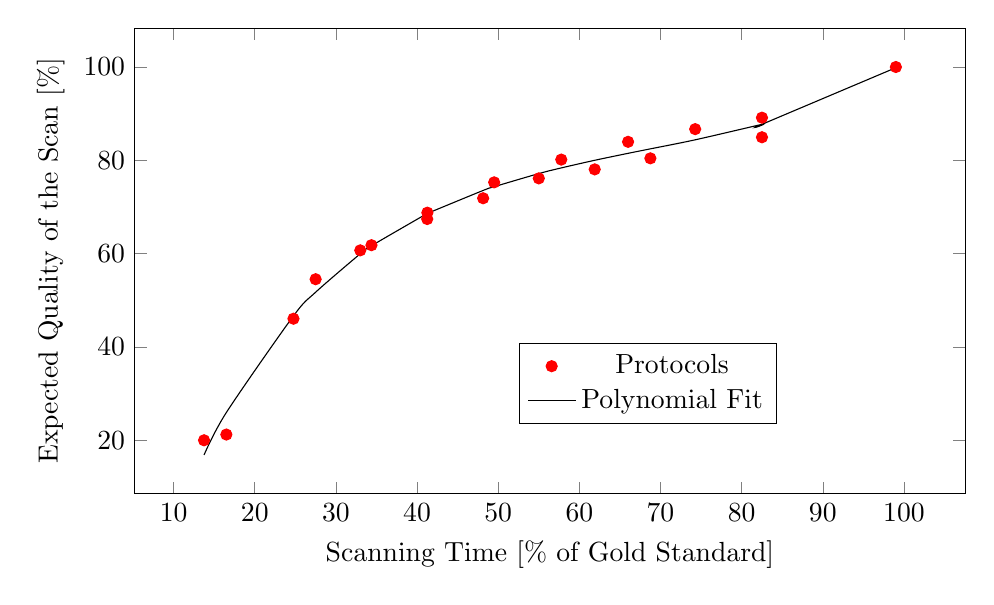
\begin{tikzpicture}

% defining custom colors
\definecolor{mycolor1}{rgb}{0,0.5,0}

\begin{axis}[%
	width=\linewidth,
	height=0.618\linewidth,
%	title={QualityPlot},%
	xlabel={Scanning Time [\%\ of Gold Standard]},%
	ylabel={Expected Quality of the Scan [\%]},%
	]

% Protocols
\addplot [ color = red, only marks, mark = *] 
coordinates{
 (13.7508,20) (16.5009,21.2284) (24.7703,46.0522) (27.5016,54.5201) (33.0019,60.7072) (34.3801,61.8107) (41.2524,67.4167) (41.2712,68.7811) (48.1435,71.8724) (49.5028,75.28) (55.0031,76.1345) (57.7722,80.1592) (61.8943,78.0612) (66.0038,83.9645) (68.7539,80.4284) (74.2731,86.6889) (82.5047,84.9458) (82.5047,89.1421) (99.0057,100)
};

% Line plot
\addplot [smooth, solid]
coordinates{
 (13.7508,16.8548) (16.5009,25.9575) (24.7703,46.6567) (27.5016,51.7347) (33.0019,59.9714) (34.3801,61.6854) (41.2524,68.6146) (41.2712,68.6305) (48.1435,73.5452) (49.5028,74.3455) (55.0031,77.1605) (57.7722,78.3754) (61.8943,80.0091) (66.0038,81.5005) (68.7539,82.4599) (74.2731,84.3973) (82.5047,87.719) (82.5047,87.719) (99.0057,99.8565)
};

\pgfplotsset{every axis legend/.append style={
at={(0.618,0.2)},
anchor=base}}

\legend{Protocols,Polynomial Fit}%$p(x)=p_{1}x^{n}+p_{2}x^{n-1}+...+p_{n}x+p_{n+1}$}

\end{axis}

\end{tikzpicture}
%%%%%%%%%%%%%%%%%%%%%%%%%%%%%%%%%%
%\end{preview}
%\end{document}%
	\caption{Quality-Plot of 19 calculated protocols. The red dots show the expected quality of the different protocols, the black plot is a polynomial fit $p(x)$ with $n=4$ for $p(x)=p_{1}x^{n}+p_{2}x^{n-1}+\cdots+p_{n}x+p_{n+1}$. Details of these scans are shown in table~\ref{tab:protocols} and are discussed in section~\ref{sec:Results}.}%
	\label{fig:qualityplot}%
	\end{figure*}
\fi

Table~\ref{tab:protocols} provides the numbers for the 19 different protocols that have been scanned for this manuscript. Protocol A would correspond to the scanning configuration shown in figure~\ref{subfig:goldstandard3}, which would require nine independent small scans, nine independent reconstructions and stitching of the resulting small datasets into one big dataset. As shown above, we can equally satisfy the sampling theorem when enough projections are acquired for a simulated detector size that is three times the real detector size of 1024 pixels, so protocol A was omitted for this study. Including an overlap of 100 pixels between the central and the ring scan, we need to acquire $N_{B}=15419$ projections for the gold-standard protocol B ($N_{B}=3(3072+200)\frac{\pi}{2}$). All the other protocols from C--T have been linearly scaled down with a decreasing percentage of acquired total projections of the gold standard. The difference of total amount of projections resulting from this scaling to the amount of projections shown in the table arises through the fact that the amount of projections for each subscan has been chosen in such a way, that the stitching of the projections was possible, hence the small differences in total amount of scanned to total amount of calculated projections.

We were able to reduce the total acquisition time by \SI{86.25}{\percent} compared to the gold standard, as can be seen in table~\ref{tab:protocols}. All 19 protocols have been scanned, reconstructed and visualized three-dimensionally to assess the artifacts which arise through the reduction of the amount of projections. Albeit the maximally assessed reduction in scanning time by \SI{86.25}{\percent} does introduce visible artifacts in the three-dimensional reconstruction (as shown in figure~\ref{fig:BvsT2}), an automated segmentation of the airways is still possible.

%%\onecolumn
%\begin{table}
%	\centering%
%	\caption{Specification of different protocols and time used compared to gold standard. Protocol A corresponds to the Gold Standard, and would have been needed to cover the same FOV with 9 independent scans with a detector width of 1024 pixels (plus an overlap of 100 pixels), resulting in a number of projections $N_{A}=9*(1024+100)\ifhtml \pi/2 \else \frac{\pi}{2} \fi= 15890$. Protocol B corresponds to the protocol shown in figure~\ref{subfig:protocol3}, resulting in a total number of projections of $N_{B} = 3(3072+200)\ifhtml \pi/2 \else \frac{\pi}{2} \fi= 15419$.}%
%	\label{tab:protocols}%
%	\begin{tabular*}{\textwidth}{r@{\extracolsep\fill}ccccccc}%
%	\toprule%
%		Protocol & A & B & C & D & E & F & G \\%
%		\midrule%
%		Total Projections & 15890 & 15732 & 13110 & 13110 & 10925 & 11802 & 9835 \\%
%		Time [\%] & 100.00 & 99.01 & 82.50 & 82.50 & 68.75 & 74.27 & 61.89 \\%
%		\bottomrule%
%	\end{tabular*}%
%	\\%
%	\begin{tabular*}{\textwidth}{r@{\extracolsep\fill}ccccccc}%
%		Protocol & H & I & J & K & L & M & N \\%
%		\midrule%
%		Total Projections & 10488 & 8740 & 9180 & 7650 & 7866 & 6555 & 6558 \\%
%		Time [\%] & 66.00 & 55.00 & 57.77 & 48.14 & 49.50 & 41.25 & 41.27 \\%
%		\bottomrule%
%	\end{tabular*}%
%	\\%
%	\begin{tabular*}{\textwidth}{r@{\extracolsep\fill}cccccc}%
%		Protocol & O & P & Q & R & S & T \\%
%		\midrule%
%		Total Projections & 5463 & 5244 & 4370 & 3936 & 2622 & 2185 \\%
%		Time [\%] & 34.38 & 33.00 & 27.50 & 24.77 & 16.50 & 13.75 \\%
%		\bottomrule%
%	\end{tabular*}%
%\end{table}%
%%\twocolumn

\begin{table}
	\caption{Specification of different protocols and time used compared to gold standard. Protocol A corresponds to the Gold Standard, and would have been needed to cover the same FOV with 9 independent scans with a detector width of 1024 pixels (plus an overlap of 100 pixels), resulting in a number of projections $N_{A}=9*(1024+100)\ifhtml \pi/2 \else \frac{\pi}{2} \fi= 15890$. Protocol B corresponds to the protocol shown in figure~\ref{subfig:protocol3}, resulting in a total number of projections of $N_{B} = 3(3072+200)\ifhtml \pi/2 \else \frac{\pi}{2} \fi= 15419$.}%
		\label{tab:protocols}%
	\centering%
	\begin{tabular}{rccccc}%
		Protocol & $s_{1}$ & $s_{2}$ & $s_{3}$ & $\sum s_{1}:s_{3}$ & Time [\%] \\%
	\hline%
		A &      &      &      & 15890 & 100.00 \\%
		B & 5244 & 5244 & 5244 & 15732 & 99.01 \\%
		C & 5244 & 2622 & 5244 & 13110 & 82.50 \\%
		D & 4370 & 4370 & 4370 & 13110 & 82.50 \\%
		E & 4370 & 2185 & 4370 & 10925 & 68.75 \\%
		F & 3934 & 3934 & 3934 & 11802 & 74.27 \\%
		G & 3934 & 1967 & 3934 &  9835 & 61.89 \\%
		H & 3496 & 3496 & 3496 & 10488 & 66.00 \\%
		I & 3496 & 1748 & 3496 &  8740 & 55.00 \\%
		J & 3060 & 3060 & 3060 &  9180 & 57.77 \\%
		K & 3060 & 1530 & 3060 &  7650 & 48.14 \\%
		L & 2622 & 2622 & 2622 &  7866 & 49.50 \\%
		M & 2622 & 1311 & 2622 &  6555 & 41.25 \\%
		N & 2186 & 2186 & 2186 &  6558 & 41.27 \\%
		O & 2185 & 1093 & 2185 &  5463 & 34.38 \\%
		P & 1748 & 1748 & 1748 &  5244 & 33.00 \\%
		Q & 1748 &  874 & 1748 &  4370 & 27.50 \\%
		R & 1312 & 1312 & 1312 &  3936 & 24.77 \\%
		S &  874 &  874 &  874 &  2622 & 16.50 \\%
		T &  874 &  437 &  874 &  2185 & 13.75 \\%
	\end{tabular}%
\end{table}

\subsection{Batch Acquisition of the Protocols}%
All subscans of each protocol have been scanned without any user intervention, except input of the sample name at the start of the batch-scan. All parameters such as sample-position in relation to the beam, rotation angles and amount of projections to obtain for the subscans have been set in a preference-file. For all 19 scanned protocols (B--T) the sample on the sample holder has not been touched, so that a direct comparison of the reconstructed slices is possible.

After acquisition of the three subscans per protocol, custom MATLAB functions read the parameters of the single subscans (e.g.\ sample name, amount of subscans, amount of dark and flat images) as well as the desired output-name and -suffix and performs all necessary calculations like loading of the correct projections from each subscan, normalizing, interpolation, cutline detection and correct stitching of the images into wide field projections. Exemplary results can be seen in figure~\ref{fig:subscans} and \ref{fig:merge-proj}.

Using the Radon transformation~\cite{Radon1917}, the corrected and merged projections were transformed into so-called sinograms, where the $n$\textsuperscript{th} is composed of the $n$\textsuperscript{th} line of every corrected projection. One sinogram thus contains as many rows as the amount of obtained corrected projections---the angular steps---and as many columns as the width of the merged projection images, thus covering an increased FOV. Each sinogram corresponds to one slice of the tomographic dataset. The $n$\textsuperscript{th} slice of the tomographic scan was reconstructed from the $n$\textsuperscript{th} sinogram using an FFT-based gridrec~\cite{Dowd1999} algorithm.

The merged projections were reconstructed on a 20-node server farm (five \SI{64}{\bit} Opteron machines with 4 cores and \SI{8}{\giga\byte} RAM each). The reconstructions result in an image stack covering a large sample volume of 2793$\times$2793$\times$1024 pixels, an approximately nine-fold increase from the standard volume of 1024$\times$1024$\times$1024 pixels for one single scan.